%%%%%%%%%%%%%%%%%%%%%%%%%%%%
%% Razor boost motivation %%
%%%%%%%%%%%%%%%%%%%%%%%%%%%%

% put text from note and expand.
% look at emails from Harrison and Maurizio

The CERN LHC (Chapter~\ref{chap:LHC}) has provided data sufficient to conduct a large variety of
searches for physics beyond the standard model.
As explained in Chapters~\ref{chap:beyond_standard_model} and \ref{chap:supersymmetry},
supersymmetry is among the best-motivated candidates for new physics and predicts the existence of
supersymmetric partners for each of the standard model particles.  
Scenarios with non-degenerate supersymmetric particle spectra, with cross sections as low as
${\sim}1$~fb, have been explored in many final states~\cite{CMS-PAS-SUS-13-020}; however, as yet no
traces of new physics have been found.  

Recently, the focus of searches has turned towards natural SUSY, in which the Higgs boson mass can
be stabilized without excessive fine tuning. Natural SUSY requires the existence of a light top
squark, $\stopone$, and a somewhat light gluino, $\tilde{g}$, while accommodating mass scales for
other supersymmetric particles that are beyond the direct reach of current LHC data.  
More detailed information on natural supersymmetry can be found in
Section~\ref{sec:susy_natural_susy}. 
The possibility that the top squark could be light has motivated several searches by the CMS and
ATLAS
collaborations~\cite{Aad:2013ija,Aad:2014qaa,Aad:2014bva,Aad:2014kva,Aad:2014kra,Chatrchyan:2013xna,
Chatrchyan:2013mya,Khachatryan:2014doa} for the direct production of top squarks. The sensitivity of
many of these searches, however, diminishes when the mass of the top squark approaches that of the
lightest SUSY particle (LSP), assumed in the remainder of this thesis to be the lightest neutralino,
$\lsp$. Searches looking specifically for $\stopone \rightarrow t \lsp$ also become less sensitive
when the mass difference, $\Delta m$, between the top squark and the LSP is comparable to the top
quark mass, $m_t$. 
These gaps in the sensitivity are illustrated in Fig.~\ref{fig:boost_story_motivation}, which shows
the general form of the exclusion limits for direct stop production, on the
($m_{\stopone},m_{\lsp}$) plane. 
Let us now examine the three regions, shown on the figure with coloured ellipses, where general
searches lack sensitivity, in order to determine why these regions are hard to probe, and whether we
can find a strategy to deal with the issues. 

\begin{figure}[htpb]
  \centering
  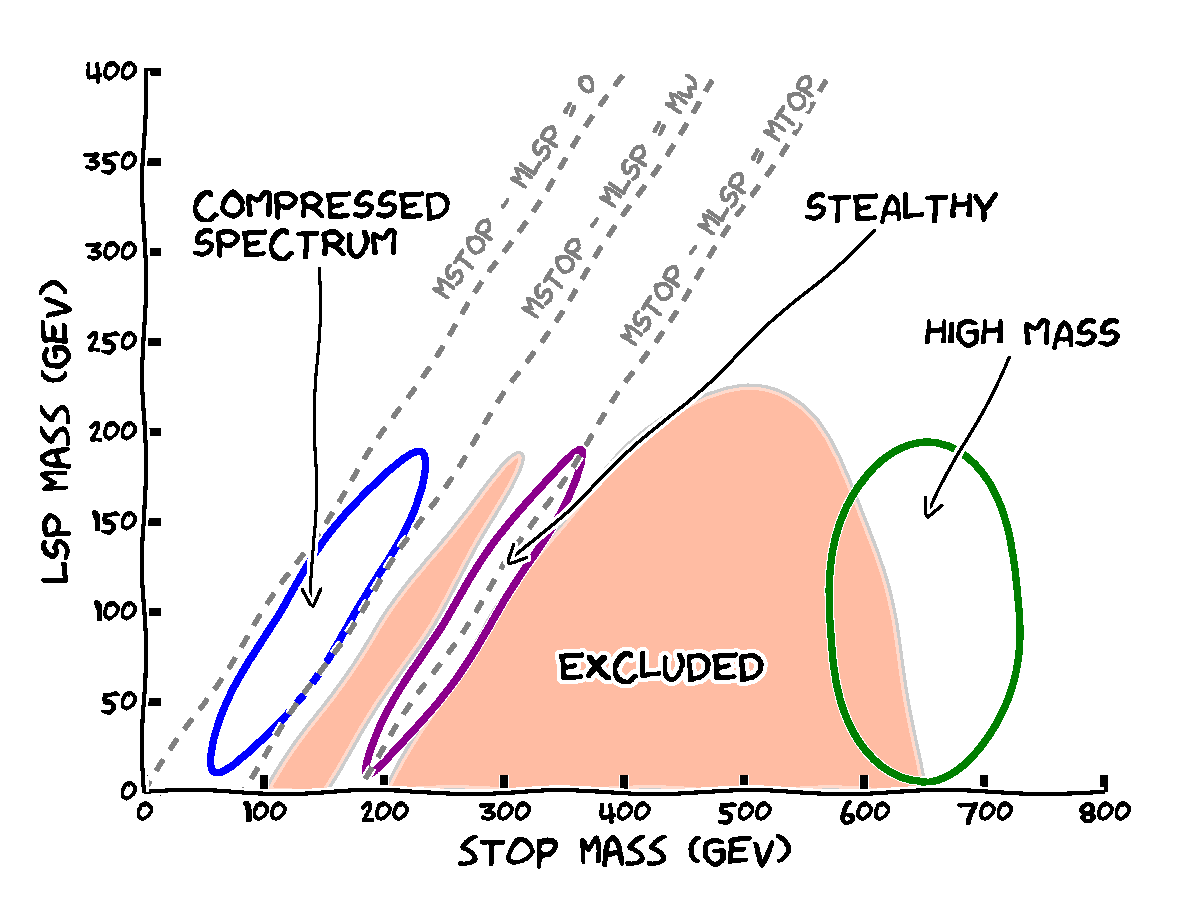
\includegraphics[width=0.8\textwidth]{figures/razor_motivation/story_boost_motivation}
  \caption{General form of the exclusion limits for direct stop production on the
($m_{\stopone},m_{\lsp}$) plane. The red shaded area is the approximate region that has been
excluded by a range of searches. The three coloured ellipses indicate the regions that are hard to
probe: the compressed spectra, stealthy top squark scenario and high mass top squarks.
  \label{fig:boost_story_motivation}}
\end{figure}

\paragraph{Compressed scenario}
In general, models with mass spectra featuring small mass splittings are called \textit{compressed
scenarios} or \textit{compressed spectra}. This case thus corresponds to the left-most gap in
Fig.~\ref{fig:boost_story_motivation}, where $\Delta m$ is very small, smaller than the $\W$ boson
mass in particular. 
In this scenario, the top squark decays to the LSP and other soft decay products, either resulting
from the loop-induced decay $\stopone \rightarrow c \lsp$, or from the four-body decay $\stopone
\rightarrow \cPqb f \bar{f} \lsp$. These soft decay products, jets and/or leptons, are difficult to
detect. They are hard to reconstruct, and when reconstructed they often fall below the \pt
thresholds that define the objects. 
Therefore, in order to be sensitive to such processes, one should not rely on the presence of
these objects, but rather on something else, such as the presence of jets from initial state
radiation (ISR). Both ATLAS and CMS have performed searches using this
technique~\cite{CMS-PAS-SUS-13-009,Aad:2014nra}. 

\paragraph{Stealthy stop scenario}
The scenarios where $\Delta m\,{\approx}\, m_t$, are often referred to as \textit{stealthy}
scenarios. The reason for this is that when $\Delta m$ approaches the top mass, the signature of
top squark production is very similar to that of standard model $t\bar{t}$ production,
which has a much higher cross section. Consequently, the signal from direct stop production is
hidden underneath a much larger $t\bar{t}$ background. An alternate way to approach stealthy stops
is, for instance, to assume that the heavy top squark $\stoptwo$ is also accessible at the LHC, and
decays to the $\stopone$ via either a Higgs or $\cPZ$ boson~\cite{Khachatryan:2014doa}. This
results in a longer decay chain, which provides extra handles, such as additional $\cPqb$ quarks or
leptons. 

\paragraph{High mass scenario}
The last gap that is present in the sensitivity of searches for the direct production of top squark
pairs, is the high mass region. In this region the signature is actually very striking, with
usually large hadronic activity and/or missing transverse momentum. The problem lies in the rather
low expected cross section for direct stop production at 8\TeV. We would need much more data than
the $20\fbinv$ that is available to detect this process. 
Of course, with the restart of the LHC at 13\TeV centre-of-mass energy fast approaching, we can
expect to close part of this gap very soon.

\paragraph{}
Apart from the approaches mentioned above, there is another option to tackle the compressed and
stealthy scenarios, namely, looking for top squarks in gluino decays. This is exactly the focus of
the razor boost analysis. 
Specifically, we consider gluino pair production in which the gluino decays to a top squark and a
top quark, $\tilde{g} \rightarrow t \stopone$. In the models considered, largely motivated by
natural supersymmetry, the gluino has a mass around 1-1.5 \TeV and the lighter top squark has a mass
of a few hundred \GeV. Owing to the significant mass gap presumed to exist between the gluino and
the top squark, the top quark from the gluino to top squark decay will receive a large boost.  
The top squark then decays to $c \lsp$ for small $\Delta m$, or to $t \lsp$ for $\Delta m
\,{\approx}\, m_t$. Four-body decays of the top squark are not considered here. 

The simplified models (see Section~\ref{sec:susy_sms} for more information) corresponding to the
decays $\tilde{g} \rightarrow t \stopone$, followed by either $\stopone \rightarrow c \lsp$ or
$\stopone \rightarrow t \lsp$, are called \textit{T1ttcc} and \textit{T1t1t}, respectively, and
illustrated in the diagrams in Fig.~\ref{fig:T1ttcc_T1t1t_diagrams}. For comparison we show in
Fig.~\ref{fig:T2tt_diagram} the diagram for the \textit{T2tt} simplified model, corresponding to
direct top squark production in which the top squark decays to $t \lsp$. 

As the analysis described in this thesis is the first analysis within CMS to explicitly probe
gluino-mediated production of top squark pairs decaying as $\stopone \rightarrow c \lsp$, it
provides new information about the viability of natural SUSY. 

\begin{figure}
  \centering
  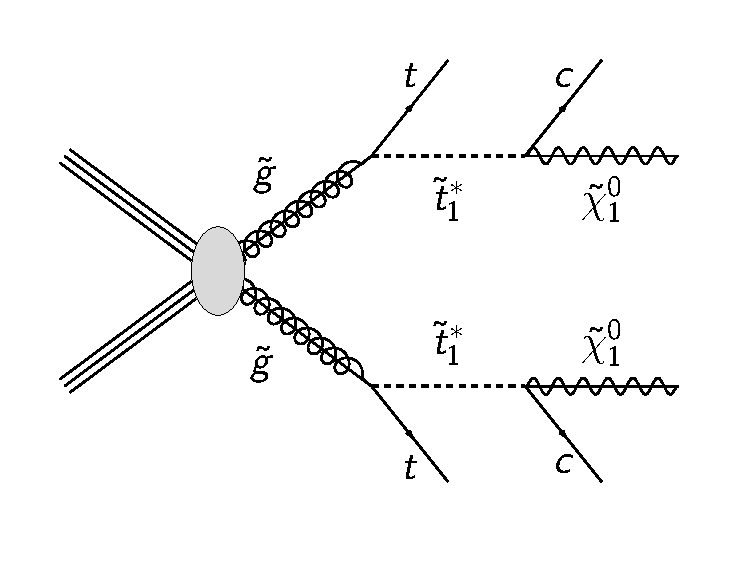
\includegraphics[width=0.48\textwidth,clip=true,trim=0 0.7cm 0 0]
{figures/razor_interpretation/T1ttcc}
  ~
  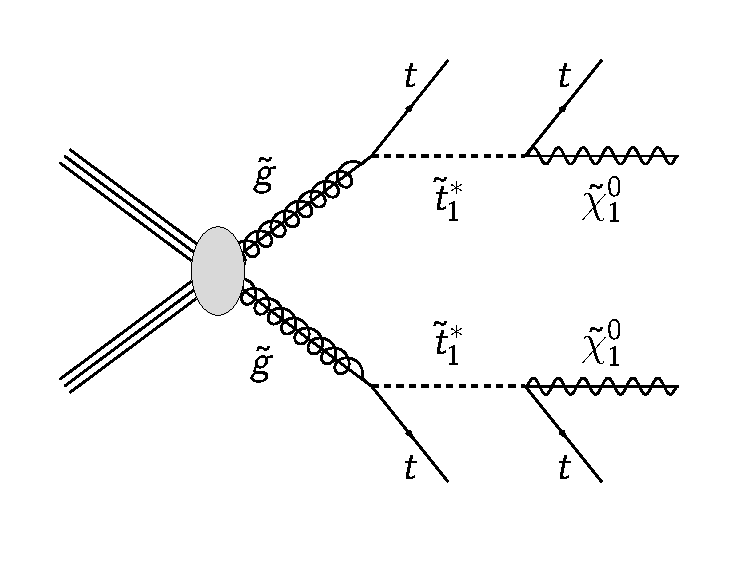
\includegraphics[width=0.48\textwidth,clip=true,trim=0 0.7cm 0 0]
{figures/razor_interpretation/T1t1t}
  \caption{Diagram illustrating the T1ttcc (left) and T1t1t (right) simplified models.
  \label{fig:T1ttcc_T1t1t_diagrams}}
\end{figure}

\begin{figure}
  \centering
  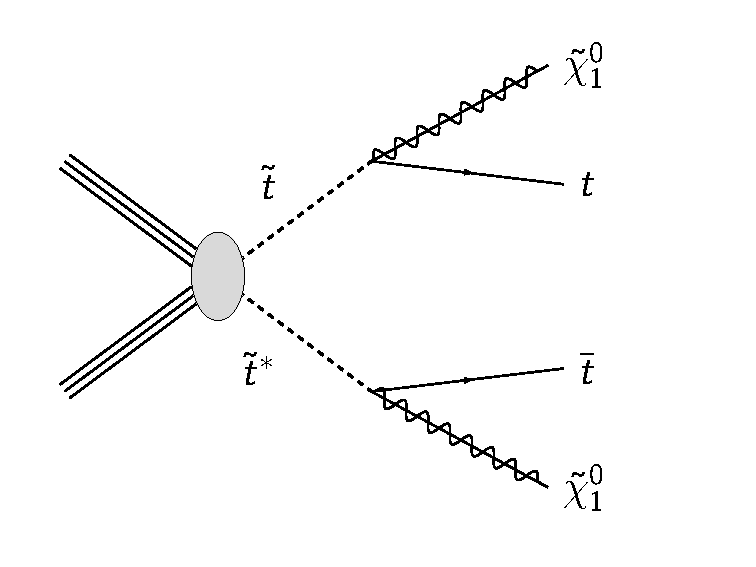
\includegraphics[width=0.48\textwidth,clip=true,trim=0 0.7cm 0 0]{figures/razor_motivation/T2tt}
  \caption{Diagram illustrating the T2tt simplified model.
  \label{fig:T2tt_diagram}}
\end{figure}


